\documentclass[12pt,chapters,notitlepage,pscyr]{hedwork}
\usepackage[utf8]{inputenc}
\usepackage[russian]{babel}
\usepackage{fourier-orns}

\makeatletter
\renewcommand{\@chapapp}{Лекция}
\makeatother

\let\labelitemi\labelitemii
\let\labelitemii\textbullet

\begin{document}
  \begin{titlepage}
    \vspace*{25em}
    \center
    \Large
    \rule[.5ex]{6em}{.5pt} \decothreeleft \rule{1em}{0pt}
    \decosix \rule{1em}{0pt}
    \decothreeright\ \rule[.5ex]{6em}{.5pt} \\[2ex]
    
    Конспект лекций по социологии \\[1.5ex]
    
    \rule{18.2em}{.5pt}
  \end{titlepage}
  
  \documentclass[pscyr,10pt]{hedlab}
\usepackage[russian]{babel}
\usepackage{graphicx}
\graphicspath{{plots/}}
\usepackage{multirow}

\labnum{1}
\labname{Технологии параллельного программирования для наиболее
распространенных параллельных архитектур}
\student{Голубев~А.~В., Чечеткин~И.~А.}

\begin{document}
  \makeheader
  
  \begin{center}
    \textbf{Begin}
  \end{center}
  
  \begin{table}[h!]
    \center
    \begin{tabular}{|C{.05}|*{8}{C{.09}|}} \hline
      count & normal & omp & \multicolumn{2}{c|}{mpi-2} &
        \multicolumn{4}{c|}{mpi-4} \\ \hline
      \( 10^1 \) & \( 4,70 \cdot 10^{-5} \) &
        \( 1,80 \cdot 10^{-3} \) &
        \( 5,90 \cdot 10^{-4} \) & \( 6,02 \cdot 10^{-4} \) &
        \( 8,64 \cdot 10^{-4} \) & \( 1,02 \cdot 10^{-3} \) &
        \( 1,19 \cdot 10^{-3} \) & \( 1,19 \cdot 10^{-3} \) \\ \hline
      \( 10^2 \) & \( 4,45 \cdot 10^{-4} \) &
        \( 1,72 \cdot 10^{-3} \) &
        \( 6,32 \cdot 10^{-4} \) & \( 6,45 \cdot 10^{-4} \) &
        \( 1,11 \cdot 10^{-3} \) & \( 9,83 \cdot 10^{-4} \) &
        \( 1,17 \cdot 10^{-3} \) & \( 1,18 \cdot 10^{-3} \) \\ \hline
      \( 10^4 \) & \( 4,46 \cdot 10^{-2} \) &
        \( 3,03 \cdot 10^{-2} \) &
        \( 6,27 \cdot 10^{-3} \) & \( 6,35 \cdot 10^{-3} \) &
        \( 5,17 \cdot 10^{-3} \) & \( 5,07 \cdot 10^{-3} \) &
        \( 6,36 \cdot 10^{-3} \) & \( 6,26 \cdot 10^{-3} \) \\ \hline
      \( 10^6 \) & \( 6,43 \) &
        \( 1,69 \) &
        \( 1,73 \) & \( 1,72 \) &
        \( 1,63 \) & \( 1,62 \) & \( 1,62 \) & \( 1,63 \) \\ \hline
      \( 10^7 \) & \( 64,26 \) &
        \( 16,15 \) &
        \( 16,50 \) & \( 16,58 \) &
        \( 16,21 \) & \( 16,20 \) & \( 16,21 \) & \( 16,29 \) \\ \hline
    \end{tabular}
  \end{table}
  
  \begin{figure}[h!]
    \center
    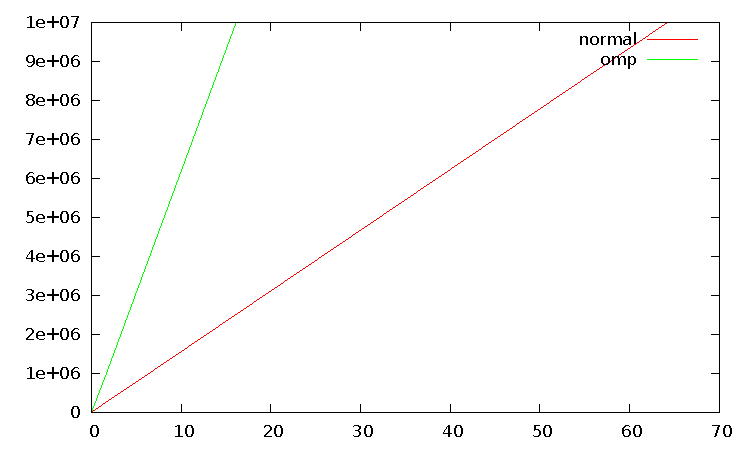
\includegraphics[width=.47\textwidth]{omp} \hspace{2em}
    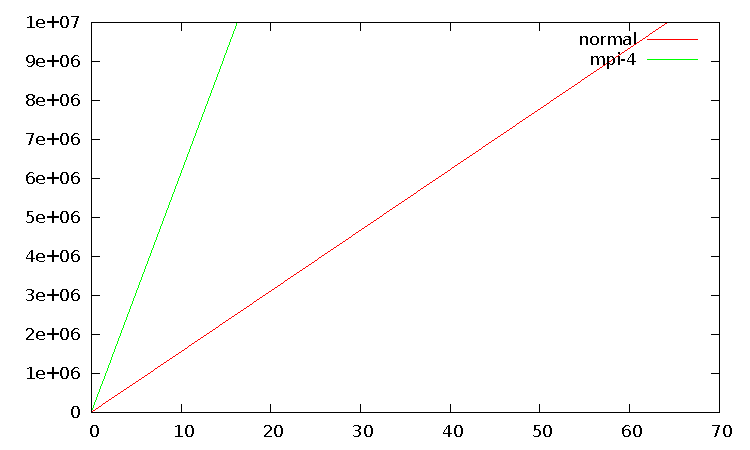
\includegraphics[width=.47\textwidth]{mpi} \\
    \parbox{.47\textwidth}{\center OpenMP} \hspace{2em}
    \parbox{.47\textwidth}{\center MPI}
  \end{figure}
  
  \begin{center}
    \textbf{Division}
  \end{center}
  
  \begin{table}[h!]
    \center
    \begin{tabular}{|C{.05}|*{8}{C{.09}|}} \hline
      count & normal & omp & \multicolumn{2}{c|}{mpi-2} &
        \multicolumn{4}{c|}{mpi-4} \\ \hline
      \( 10^1 \) & \( 2,42 \cdot 10^{-5} \) &
        \( 2,58 \cdot 10^{-5} \) &
        \( 3,57 \cdot 10^{-4} \) & \( 3,82 \cdot 10^{-4} \) &
        \( 4,46 \cdot 10^{-4} \) & \( 6,47 \cdot 10^{-4} \) &
        \( 5,69 \cdot 10^{-4} \) & \( 6,73 \cdot 10^{-4} \) \\ \hline
      \( 10^2 \) & \( 2,40 \cdot 10^{-4} \) &
        \( 2,43 \cdot 10^{-4} \) &
        \( 4,77 \cdot 10^{-4} \) & \( 4,83 \cdot 10^{-4} \) &
        \( 5,41 \cdot 10^{-4} \) & \( 7,00 \cdot 10^{-4} \) &
        \( 9,09 \cdot 10^{-4} \) & \( 8,05 \cdot 10^{-4} \) \\ \hline
      \( 10^4 \) & \( 2,42 \cdot 10^{-2} \) &
        \( 2,43 \cdot 10^{-2} \) &
        \( 1,26 \cdot 10^{-2} \) & \( 1,25 \cdot 10^{-2} \) &
        \( 7,10 \cdot 10^{-3} \) & \( 7,20 \cdot 10^{-3} \) &
        \( 7,20 \cdot 10^{-3} \) & \( 7,18 \cdot 10^{-3} \) \\ \hline
      \( 10^6 \) & \( 2,41 \) &
        \( 2,41 \) &
        \( 1,22 \) & \( 1,21 \) &
        \( 6,31 \cdot 10^{-1} \) & \( 6,33 \cdot 10^{-1} \) &
        \( 6,34 \cdot 10^{-1} \) & \( 6,29 \cdot 10^{-1} \) \\ \hline
      \( 10^7 \) & \( 24,10 \) &
        \( 24,10 \) &
        \( 12,18 \) & \( 12,12 \) &
        \( 6,30 \) & \( 6,26 \) & \( 6,29 \) & \( 6,31 \) \\ \hline
    \end{tabular}
  \end{table}
  
  \begin{center}
    \textbf{Super Functions}
  \end{center}
  
  \begin{table}[h!]
    \center
    \begin{tabular}{|C{.05}|*{8}{C{.09}|}} \hline
      count & normal & omp & \multicolumn{2}{c|}{mpi-2} &
        \multicolumn{4}{c|}{mpi-4} \\ \hline
      \( 10^1 \) & \( 2,60 \cdot 10^{-3} \) &
        \( 2,60 \cdot 10^{-3} \) &
        \( 1,61 \cdot 10^{-3} \) & \( 1,67 \cdot 10^{-3} \) &
        \( 1,20 \cdot 10^{-3} \) & \( 1,40 \cdot 10^{-3} \) &
        \( 1,08 \cdot 10^{-3} \) & \( 1,31 \cdot 10^{-3} \) \\ \hline
      \( 10^2 \) & \( 2,60 \cdot 10^{-2} \) &
        \( 2,60 \cdot 10^{-2} \) &
        \( 1,34 \cdot 10^{-2} \) & \( 1,34 \cdot 10^{-2} \) &
        \( 6,88 \cdot 10^{-3} \) & \( 7,14 \cdot 10^{-3} \) &
        \( 6,99 \cdot 10^{-3} \) & \( 7,07 \cdot 10^{-3} \) \\ \hline
      \( 10^4 \) & \( 2,60 \) &
        \( 2,60 \) &
        \( 1,30 \) & \( 1,30 \) &
        \( 6,54 \cdot 10^{-1} \) & \( 6,54 \cdot 10^{-1} \) &
        \( 6,54 \cdot 10^{-1} \) & \( 6,54 \cdot 10^{-1} \) \\ \hline
      \( 10^6 \) & \( 263 \) &
        \( 262 \) &
        \( 129 \) & \( 130 \) &
        \( 65,9 \) & \( 65,9 \) & \( 65,9 \) & \( 65,7 \) \\ \hline
    \end{tabular}
  \end{table}
  
  \newpage
  
  \begin{center}
    \textbf{Switch}
  \end{center}
  
  \begin{table}[h!]
    \center
    \begin{tabular}{|C{.05}|*{7}{C{.09}|}} \hline
      count & omp & \multicolumn{2}{c|}{mpi-2} &
        \multicolumn{4}{c|}{mpi-4} \\ \hline
      \( 10^1 \) & \( 5,00 \cdot 10^{-5} \) &
        \( 3,45 \cdot 10^{-4} \) & \( 3,83 \cdot 10^{-4} \) &
        \( 4,69 \cdot 10^{-4} \) & \( 5,71 \cdot 10^{-4} \) &
        \( 6,75 \cdot 10^{-4} \) & \( 6,60 \cdot 10^{-4} \) \\ \hline
      \( 10^2 \) & \( 4,83 \cdot 10^{-4} \) &
        \( 5,67 \cdot 10^{-4} \) & \( 5,69 \cdot 10^{-4} \) &
        \( 7,59 \cdot 10^{-4} \) & \( 5,39 \cdot 10^{-4} \) &
        \( 7,19 \cdot 10^{-4} \) & \( 5,93 \cdot 10^{-4} \) \\ \hline
      \( 10^4 \) & \( 4,83 \cdot 10^{-2} \) &
        \( 2,18 \cdot 10^{-2} \) & \( 2,17 \cdot 10^{-2} \) &
        \( 1,19 \cdot 10^{-2} \) & \( 1,23 \cdot 10^{-2} \) &
        \( 7,20 \cdot 10^{-2} \) & \( 7,18 \cdot 10^{-2} \) \\ \hline
      \( 10^6 \) & \( 7,61 \) &
        \( 3,82 \) & \( 3,82 \) &
        \( 1,94 \) & \( 1,94 \) & \( 1,93 \) & \( 1,93 \) \\ \hline
      \( 10^7 \) & \( 76,20 \) &
        \( 38,20 \) & \( 38,19 \) &
        \( 19,30 \) & \( 19,38 \) & \( 19,29 \) & \( 19,32 \) \\ \hline
    \end{tabular}
  \end{table}
  
  \begin{center}
    \textbf{Sunlight}
  \end{center}
  
  \begin{table}[h!]
    \center
    \begin{tabular}{|*{8}{C{.1}|}} \hline
      count & omp & \multicolumn{2}{c|}{mpi-2} &
        \multicolumn{4}{c|}{mpi-4} \\ \hline
      \multicolumn{8}{|c|}{count\_of\_steps = 1} \\ \hline
      10 & \( 2,05 \cdot 10^{-6} \) &
        \( 6,03 \cdot 10^{-4} \) & \( 6,23 \cdot 10^{-4} \) &
        \( 1,17 \cdot 10^{-3} \) & \( 1,07 \cdot 10^{-3} \) &
        \( 9,13 \cdot 10^{-4} \) & \( 1,15 \cdot 10^{-3} \) \\ \hline
      10000 & \( 3,28 \cdot 10^{-5} \) &
        \( 1,04 \cdot 10^{-3} \) & \( 2,46 \cdot 10^{-3} \) &
        \( 3,94 \cdot 10^{-3} \) & \( 2,41 \cdot 10^{-3} \) &
        \( 3,00 \cdot 10^{-3} \) & \( 4,06 \cdot 10^{-3} \) \\ \hline
      1000000 & \( 8,92 \cdot 10^{-3} \) &
        \( 3,48 \cdot 10^{-2} \) & \( 1,83 \cdot 10^{-1} \) &
        \( 2,27 \cdot 10^{-1} \) & \( 8,04 \cdot 10^{-2} \) &
        \( 2,23 \cdot 10^{-1} \) & \( 2,31 \cdot 10^{-1} \) \\ \hline
      \multicolumn{8}{|c|}{count\_of\_steps = 10} \\ \hline
      10 & \( 2,05 \cdot 10^{-6} \) &
        \( 7,22 \cdot 10^{-4} \) & \( 7,48 \cdot 10^{-4} \) &
        \( 2,17 \cdot 10^{-3} \) & \( 3,72 \cdot 10^{-3} \) &
        \( 3,70 \cdot 10^{-3} \) & \( 2,05 \cdot 10^{-3} \) \\ \hline
      10000 & \( 1,22 \cdot 10^{-4} \) &
        \( 3,76 \cdot 10^{-3} \) & \( 2,27 \cdot 10^{-3} \) &
        \( 3,47 \cdot 10^{-2} \) & \( 3,88 \cdot 10^{-2} \) &
        \( 3,47 \cdot 10^{-2} \) & \( 3,56 \cdot 10^{-2} \) \\ \hline
      1000000 & \( 1,27 \cdot 10^{-2} \) &
        \( 2,92 \cdot 10^{-1} \) & \( 4,38 \cdot 10^{-1} \) &
        \( 8,32 \cdot 10^{-1} \) & \( 8,28 \cdot 10^{-1} \) &
        \( 6,85 \cdot 10^{-1} \) & \( 8,40 \cdot 10^{-1} \) \\ \hline
    \end{tabular}
  \end{table}
  
  \begin{center}
    \textbf{Solid Body}
  \end{center}
  
  \begin{table}[h!]
    \center
    \begin{tabular}{|*{8}{C{.1}|}} \hline
      count (x,~y,~z) & omp & \multicolumn{2}{c|}{mpi-2} &
        \multicolumn{4}{c|}{mpi-4} \\ \hline
      \multicolumn{8}{|c|}{count\_of\_steps = 1} \\ \hline
      5 & \( 2,95 \cdot 10^{-2} \) &
        \( 7,13 \cdot 10^{-4} \) & \( 7,46 \cdot 10^{-4} \) &
        \( 1,42 \cdot 10^{-3} \) & \( 1,35 \cdot 10^{-3} \) &
        \( 9,91 \cdot 10^{-4} \) & \( 1,38 \cdot 10^{-3} \) \\ \hline
      50 & \( 1,23 \cdot 10^{-1} \) &
        \( 5,28 \cdot 10^{-2} \) & \( 5,01 \cdot 10^{-2} \) &
        \( 4,44 \cdot 10^{-2} \) & \( 5,53 \cdot 10^{-2} \) &
        \( 4,40 \cdot 10^{-2} \) & \( 5,23 \cdot 10^{-2} \) \\ \hline
      200 & \( 8,97 \) &
        \( 2,97 \) & \( 2,76 \) &
        \( 2,86 \) & \( 3,03 \) & \( 2,90 \) & \( 2,83 \) \\ \hline
      \multicolumn{8}{|c|}{count\_of\_steps = 10} \\ \hline
      5 & \( 3,12 \cdot 10^{-4} \) &
        \( 1,11 \cdot 10^{-3} \) & \( 1,15 \cdot 10^{-3} \) &
        \( 9,89 \cdot 10^{-3} \) & \( 9,19 \cdot 10^{-3} \) &
        \( 8,66 \cdot 10^{-3} \) & \( 9,80 \cdot 10^{-3} \) \\ \hline
      50 & \( 1,25 \) &
        \( 5,18 \cdot 10^{-1} \) & \( 5,16 \cdot 10^{-1} \) &
        \( 5,33 \cdot 10^{-1} \) & \( 5,33 \cdot 10^{-1} \) &
        \( 5,33 \cdot 10^{-1} \) & \( 5,38 \cdot 10^{-1} \) \\ \hline
      200 & \( 89,70 \) &
        \( 25,98 \) & \( 26,18 \) &
        \( 27,86 \) & \( 27,76 \) & \( 27,82 \) & \( 27,78 \) \\ \hline
    \end{tabular}
  \end{table}
\end{document}
\end{document}
